\subsection{CLI Options}
\label{annex:cli-options}

\begin{table}[H]
    \begin{tabular}{|l|l|l|l|}
        \hline
        short & long      & default    & short description                                                  \\ \hline
        -i    & --input   & *required* & Path to the input image, can be a file or a directory, must be set \\ \hline
        -o    & --output  &            & Path to the output image, can be a file or a directory             \\ \hline
        -c    & --compare & false      & Compare quality of the output image with the input image           \\ \hline
        -d    & --debug   & false      & Enable debug mode                                                  \\ \hline
        -f    & --force   & false      & Force the overwrite of the output file (if it exists)              \\ \hline
        -h    & --help    & false      & Show  help message                                                 \\ \hline
        -q    & --quiet   & false      & Disable the console output                                         \\ \hline
        -r    & --ratio   & 0.5        & Set the ratio of the JPEG compression                              \\ \hline
        -t    & --test    & false      & Run the test suite                                                 \\ \hline
        -v    & --version & false      & Show version                                                       \\ \hline
    \end{tabular}
\end{table}

\begin{dinglist}{111}
    \item \texttt{input}

    The input image can be a file or a directory. If it is a directory, all the images in the directory will be compressed.
    Accepted extensions are:
    \iCode{.jpg}, \iCode{.jpeg}, \iCode{.png}, \iCode{.bmp}, \iCode{.tiff}, \iCode{.gif}, \iCode{.webp}.

    If you want to handle multiple images in the same time, you have to put all of them in a directory.
    The program will take all accepted images in this directory.
    You cannot give several files path.

    \item \texttt{output}

    The output image can be a file or a directory. If it is a directory, all the images in the input directory will be compressed and saved in the output directory.
    If the specified path does not exist, it will be created (if there is sufficient access, else it will raise an error).

    The extension has to be `.jpg` or `.jpeg` (it will be the same output for both extensions).

    You cannot give multiple output files path, only a file path or directory path.

    \item \texttt{compare}

    If this option is set, the quality of the output image will be compared with the input image.

    \item \texttt{debug}

    If this option is set, the debug mode will be enabled. This will print the debug messages in the console.

    \item \texttt{force}

    If this option is set, the output file will be overwritten if it already exists.

    \item \texttt{help}

    If this option is set, the help message will be printed in the console.

    \item \texttt{quiet}

    If this option is set, the console output will be disabled.

    \item \texttt{ratio}

    This option sets the ratio of the JPEG compression. The ratio must be a float between 0 and 1. The higher the ratio, the better the quality of the output image.

    \item \texttt{test}

    If this option is set, the test suite will be run.

    \item \texttt{version}

    If this option is set, the version of the program will be printed in the console.

\end{dinglist}

\subsection{Images}

Here are the original tests images.

\begin{figure}[H]
    \centering
    % subfigures 2 images
    \begin{subfigure}[b]{0.4\textwidth}
        \centering
        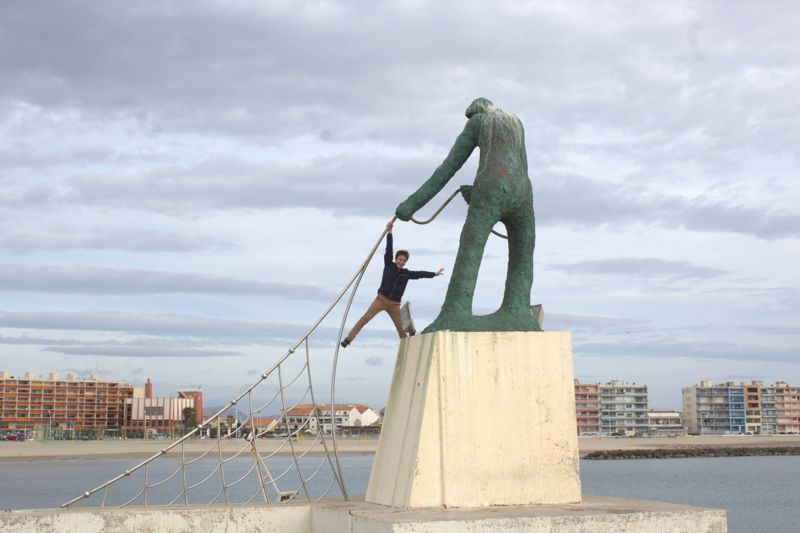
\includegraphics[width=0.9\textwidth]{src/assets/tests/tests_original.jpg}
        \caption{Original tests image}
        \label{fig:original-tests}
    \end{subfigure}
    \begin{subfigure}[b]{0.4\textwidth}
        \centering
        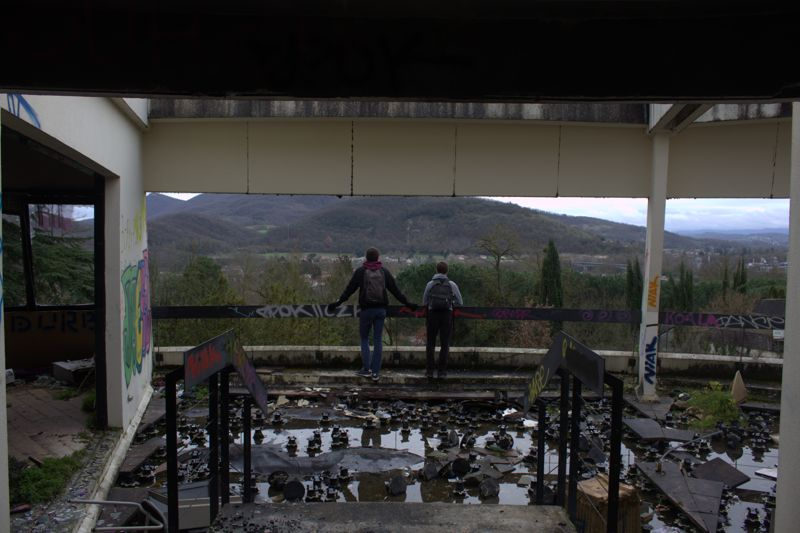
\includegraphics[width=0.9\textwidth]{src/assets/head/head_original.jpg}
        \caption{Original head image}
        \label{fig:original-head}
    \end{subfigure}
\end{figure}
